\def\fileversion{v2.25a} \def\filedate{2009/10/10}
% \iffalse  % this is a METACOMMENT !
%% Package and Class "uiucthesis2009" for use with LaTeX2e.
%
%<class|package>\NeedsTeXFormat{LaTeX2e}
%<class>\ProvidesClass{uiucthesis2009}
%<package>\ProvidesPackage{uiucthesis2009}
%<class|package>         [\filedate\ \fileversion\ UIUC Thesis (PJC)]
%
%<*driver>
\documentclass{ltxdoc}
\begin{document}
\title{The \textsf{uiucthesis2009} class
       \thanks{This file has version number \fileversion,
       last revised \filedate.}}
\author{Charles Kiyanda\\charles@kiyanda.com\\(Adapted from version 2.25, 2005/03/25 by Peter Czoschke\\Updated in 2007 by Tim Head.)}
\date{\filedate}
\maketitle
\DocInput{uiucthesis2009.dtx}
\end{document}
%</driver>
% \fi
%
% \CheckSum{1164}
%
% \MakeShortVerb{\|}
%
% \def\pkg#1{\textsf{#1}}
% \def\env#1{\textsf{#1}}
%
% \iffalse
%<*example>
% \fi
% \begin{abstract}
% Load the \pkg{uiucthesis2009} class for use with \LaTeX2e
% to produce a document that should conform
% to the format described in
% \emph{Handbook for Graduate Students Preparing to Deposit}\cite{Handbook}. (Actually
% I have checked the requirements from a grad college webpage\cite{thesisweb}.
% I believe 
% this template complies, but there is no guarantee.)
% \end{abstract}
% 
% \section{The User Interface}
%
% This section describes how to use the \pkg{uiucthesis2009} class to
% produce a thesis satisfying the format requirements of the
% Grad College at UIUC.
% I assume that you are familiar with \LaTeX, and highly
% recommend that anyone attempting to use \LaTeX\ to produce a
% thesis have access to a copy of the \LaTeX\ book\cite{Lamport}.
%
% Note that I haven't graduated yet and so I haven't taken this template
% through the ultimate test, which is to actually submit a thesis that ues it.
% I believe this template does conform to the graduate college requirement, but I am,
% \emph{in no way} guaranteeing it conforms to anything.
%
% Also, I'm writing my thesis right now as well. I don't plan to make any more changes to this
% template until I graduate. Hence, if you send me an e-mail right now asking to change some
% detail that you'd think looks better, you're likely to either
% not get a response or receive a somewhat polite ``Wait until january...'' type of response.
% If you firmly believe this template does not conform to the graduate college requirements, be
% very precise and I might look at it. It's just the way it is right now, I'm afraid...
% 
% \subsection{Using \pkg{uiucthesis2009}}
%
% To write a thesis, you load the UIUC thesis definitions
% by loading the \pkg{uiucthesis2009} class at the beginning of
% your \LaTeX\ document with the |\documentclass| command.
% For example,
% \begin{quote} \hrule \begin{verbatim}
\documentclass[edeposit,fullpage]{uiucthesis2009}
% \end{verbatim} \hrule \end{quote}
% \iffalse
%<example>
% \fi
%
% \DescribeMacro{[draftthesis]}
% \DescribeMacro{[fancy]}
% \DescribeMacro{[fullpage]}
% The \pkg{uiucthesis2009} class provides a number of options.
% The |[draftthesis]| option causes each page to have a header
% proclaiming the document to be a draft copy, along with the
% current time and date.
% It also omits the copyright page and prints out any marginal notes
% added with the |\note| macro.
% The |[fancy]| style option produces slightly fancier chapter headings.
% The |[fullpage]| style option makes the margins as small as the
% format requirements allow and uses double-spacing for the text.
% Because wide text columns are generally
% considered harder on the reader
% this is not the default, but is provided as an option because people
% seem to want it.
% The |[fancy]| and |[fullpage]| options are incompatible---choose
% one or the other.
%
% \DescribeMacro{[proquest]}
% The |[proquest]| option is meant to be used when you are ready to deposit your thesis.
% For doctorates, the Grad College requires the submission of a specially
% formatted abstract for the ProQuest publication service. To produce this
% abstract, include the |[proquest]| option and reprocess your file. Everything
% in your \LaTeX\ document will be ignored except the contents of the \env{abstract}
% environment, which are printed out in the format required. Once the option is
% removed from the |\documentclass| command, you can reprocess your thesis as
% normal (the auxiliary files should be intact). To use this option, the name
% of your thesis advisor needs to be specified with the |\advisor| command (see
% below).
%
% \DescribeMacro{[edeposit]}
% Use the |[edeposit]| option if you are depositing your thesis electronically. The title page
% used to be different, but the requirement appears to have been harmonized since. The page 
% numbering is slightly different since the committee
% approval form is not included with your thesis. (The page numbering change is currently the
% only difference of thet edeposit option.  You
% must specify your committee members with the |\committee| command (see below).
%
% \DescribeMacro{[offcenter]}
% The |[offcenter]| option adds 1/2 inch to the left margin of all pages and takes
% away 1/2 inch to the text width, leaving a 1.5in left margin and a 1in right margin.
% I believe this setting satisfies the pre-2009 requirement by the grad college to
% have a 1.5in margin for binding. It should also allow you more room for binding
% if you need it. The new requirement is a minimum 1in margin all around and the 
% |[fullpage]| option without the |[offcenter]| option should achieve this goal.
%
% This can now be done to allow some extra space there for binding purposes, or
% if you use the |[fancy]| option, to allow for more space for the chapter
% numbers at the left side of the page.
% In past versions of \pkg{uiucthesis2009} (the name used was simply uiucthesis)
% , the |[fancy]| option did this by default.
% This version uses symmetric margins by default, even with the
% |[fancy]| option. If you have a lot of chapters (i.e., more than 9), your chapter
% numbers may spill into
% the 1 inch margin required by the Grad College without using this option.
%
% \DescribeMacro{[centerchapter]}
% Normally, the chapter headings are all left-justified on the opening page of
% each chapter. These headings can all be centered by using the |[centerchapter]|
% option for the class. This option is not recommended for use with the |[fancy]|
% option.
%
% \subsection{The Title Page}
%
% The |\maketitle| command is redefined so that it creates a
% title page with the correct format for a thesis at UIUC.
%
% \DescribeMacro{\phdthesis}
% \DescribeMacro{\otherdoctorate}
% \DescribeMacro{\msthesis}
% \DescribeMacro{\othermasters}
% \DescribeMacro{\department}
% \DescribeMacro{\college}
% Use the |\phdthesis| or |\msthesis| to set the correct thesis type.
% If your thesis isn't for a ``Ph.D.'' or ``M.S.'', you can specify
% your degree with either\\
% |\otherdoctorate{|\meta{degree name}|}{|\meta{abbreviation}|}| or\\
% |\othermasters{|\meta{degree name}|}{|\meta{abbreviation}|}|.\\
% For example, specifying |\phdthesis| is equivalent to giving the command\\
% |\otherdoctorate{Doctor of Philosophy}{Ph.D.}|.\\
% The default thesis type is |\phdthesis|. Set your department with\linebreak
% |\department{|\meta{department}|}|. This defines the field your degree
% will be in, so leave out ``Department of.''
% The default department is ``Computer Science''.
% Define your college with |\college{|\meta{college}|}|.
% The default is college is ``Graduate College'';
% you shouldn't need to change it.
%
% \DescribeMacro{\schools}
% Use |\schools{|\meta{school list}|}| to list the previous degrees
% you have received and the schools that you received them from.
% Separate multiple degrees with |\\|.
%
% \DescribeMacro{\degreeyear}
% Use |\degreeyear{|\meta{year}|}| to define the year in which
% you will receive your degree.  The default is the current year.
%
% \DescribeMacro{\advisor}
% \DescribeMacro{\adviser}
% Use |\advisor{|\meta{advisor name}|}| or |\adviser{|\meta{advisor name}|}|
% to specify the name of your
% advisor. This is needed to produce the ProQuest abstract
% (see the |[proquest]| option above). You only need to submit a
% ProQuest abstract if you are a doctoral candidate.
%
% \DescribeMacro{\committee}
% Use |\committee{|\meta{committee members}|}| to specify the members
% of your committee and their titles as you want them to appear on the
% title page. Separate members with |\\|. This is needed for
% all forms of thesis submission. To respect the graduate college guidelines,
% you must use the full title of each committee members. The committee chair should
% appear first with the designation ``,chair''. Your thesis adviser should appear second
% with the title ``,Director of Research''. See the graduate college website for details.
%
% \DescribeMacro{\volume}
% The |\volume| macro provides nominal support for very long theses that must
% be broken up into multiple volumes. Use |\volume{|\meta{number}|}|
% to specify the volume number (a single arabic numeral). All this macro
% does is place the word VOLUME with the number you specify on the title
% page. You have to take care of what appears in each volume. The easiest
% way to do this is to create two separate source files, one for each
% volume.
%
% Here's how to produce an example similar to that in \cite{Handbook}.
% \begin{quote} \hrule \begin{verbatim}
\begin{document}

\title{Coffee Consumption of Graduate Students \\
       Trying to Finish Dissertations}
\author{Juan Valdez}
\department{Food Science}
\schools{B.A., University of Columbia, 1981\\
         A.M., University of Illinois at Urbana-Champaign, 1986}
\phdthesis
\advisor{Java Jack}
\degreeyear{1994}
\committee{Professor Prof Uno, Chair\\Professor Prof Dos, Director of Research\\Assistant Professor Prof Tres\\Adjunct Professor Prof Quatro}
\maketitle
% \end{verbatim} \hrule \end{quote}
% \iffalse
%<example>
% \fi
%
% \subsection{Front Matter}
%
% \DescribeMacro{\frontmatter}
% Typically, a thesis might have an Abstract, a Dedication, some
% Acknowledgments, and a Preface before the Table of Contents.
% Use the |\frontmatter| command to start this preliminary section
% of the thesis.
% The |\frontmatter| command sets the page number of the next page
% to roman numeral iii (or ii if the |[edeposit]| option is used).
% (The title page is page i, and the certificate
% of committee approval, the ``red-bordered form,'' is page ii.)
%
% \DescribeEnv{abstract}
% The abstract should appear in the \env{abstract} environment. Normally,
% this just produces another chapter with |\chapter*{\abstractname}|,
% where |\abstractname| is ``Abstract'' (see User Customization below),
% but if the |[proquest]| option
% is specified, then the contents of this environment are used
% for the ProQuest abstract.
%
% \DescribeEnv{dedication}
% A dedication page can be printed with the \env{dedication} environment.
% This produces a separate page with the dedication centered horizontally
% and vertically, with the text in italics.
%
% After this front matter comes the Table of Contents,
% List of Tables, List of Figures, etc.  Use the standard \LaTeX\
% commands |\tableofcontents|, |\listoftables|, |\listoffigures|, etc.,
% to generate them.
% In the \pkg{uiucthesis2009} format these lists are all single spaced.
%
% \DescribeEnv{symbollist}
% \DescribeEnv{symbollist*}
% Optionally, these tables can be followed by a List of Abbreviations and/or
% List of Symbols. Introduce these with the |\chapter| command. To aid in
% making these lists, the \env{symbollist} and \env{symbollist*} environments are
% defined in \pkg{uiucthesis2009}. These environments produce a two-column list
% as illustrated below. By default the left column is 1 inch wide but can
% be specified with an optional argument. In the starred environment, the left
% column is left-justified, otherwise it is centered. See the example below.
%
% Here's an example of what the front matter of a typical
% thesis looks like.  First comes the Abstract and the Dedication, both of
% which are optional.
% \begin{quote} \hrule \begin{verbatim}
\frontmatter

%% Create an abstract that can also be used for the ProQuest abstract.
%% Note that ProQuest truncates their abstracts at 350 words.
\begin{abstract}
This is a comprehensive study of caffeine consumption by graduate
students at the University of Illinois who are in the very final
stages of completing their doctoral degrees. A study group of six
hundred doctoral students\ldots.
\end{abstract}

%% Create a dedication in italics with no heading, centered vertically
%% on the page.
\begin{dedication}
To Father and Mother.
\end{dedication}

%% Create an Acknowledgements page, many departments require you to
%% include funding support in this.
\chapter*{Acknowledgments}

This project would not have been possible without the support of
many people. Many thanks to my adviser, Lawrence T. Strongarm, who
read my numerous revisions and helped make some sense of the
confusion. Also thanks to my committee members, Reginald Bottoms,
Karin Vegas, and Cindy Willy, who offered guidance and support.
Thanks to the University of Illinois Graduate College for awarding
me a Dissertation Completion Fellowship, providing me with the
financial means to complete this project. And finally, thanks to
my husband, parents, and numerous friends who endured this long
process with me, always offering support and love.

%% The thesis format requires the Table of Contents to come
%% before any other major sections, all of these sections after
%% the Table of Contents must be listed therein (i.e., use \chapter,
%% not \chapter*).  Common sections to have between the Table of
%% Contents and the main text are:
%%
%% List of Tables
%% List of Figures
%% List Symbols and/or Abbreviations
%% etc.

\tableofcontents
\listoftables
\listoffigures
% \iffalse
%<example>
% \fi
% \end{verbatim} \hrule \end{quote}
%
% If you want a List of Symbols or Abbreviations, you can do so as follows:
% \begin{quote} \hrule \begin{verbatim}
%% Create a List of Abbreviations. The left column
%% is 1 inch wide and left-justified
\chapter{List of Abbreviations}

\begin{symbollist*}
\item[CA] Caffeine Addict.
\item[CD] Coffee Drinker.
\end{symbollist*}

%% Create a List of Symbols. The left column
%% is 0.7 inch wide and centered
\chapter{List of Symbols}

\begin{symbollist}[0.7in]
\item[$\tau$] Time taken to drink one cup of coffee.
\item[$\mu$g] Micrograms (of caffeine, generally).
\end{symbollist}
% \end{verbatim} \hrule \end{quote}
% \iffalse
%<example>
% \fi
%
% \subsection{Main Matter}
%
% \DescribeMacro{\mainmatter}
% Begin the main body of your thesis with the |\mainmatter| command.
% It resets the page number to arabic numeral 1.
% You can now use any of the commands defined by the
% the book document class to write your thesis.
%
% In the following example, each of the chapters
% has been broken out into separate files that are inserted into
% this main file with the |\include| command.  This allows the
% thesis to be proofed quickly while it is being revised with
% the |\includeonly| command.  To provide an example of what the
% chapter headings look like, one chapter has been explicitly
% coded. (Try recompiling the example file with the |[fancy]|
% option instead of |[fullpage]| to see the effect.)
%
% \begin{quote} \hrule \begin{verbatim}
\mainmatter
% Sample chapter to test margins
\chapter{This world}
\section{Of the Nature of Flatland}


I call our world Flatland, not because we call it so, but to make its
nature clearer to you, my happy readers, who are privileged to live in
Space.

Imagine a vast sheet of paper on which straight Lines, Triangles,
Squares, Pentagons, Hexagons, and other figures, instead of remaining
fixed in their places, move freely about, on or in the surface, but
without the power of rising above or sinking below it, very much like
shadows--only hard with luminous edges--and you will then have a pretty
correct notion of my country and countrymen.  Alas, a few years ago, I
should have said "my universe:"  but now my mind has been opened to
higher views of things.

In such a country, you will perceive at once that it is impossible that
there should be anything of what you call a "solid" kind; but I dare
say you will suppose that we could at least distinguish by sight the
Triangles, Squares, and other figures, moving about as I have described
them.  On the contrary, we could see nothing of the kind, not at least
so as to distinguish one figure from another.  Nothing was visible, nor
could be visible, to us, except Straight Lines; and the necessity of
this I will speedily demonstrate.

Place a penny on the middle of one of your tables in Space; and leaning
over it, look down upon it.  It will appear a circle.

But now, drawing back to the edge of the table, gradually lower your
eye (thus bringing yourself more and more into the condition of the
inhabitants of Flatland), and you will find the penny becoming more and
more oval to your view, and at last when you have placed your eye
exactly on the edge of the table (so that you are, as it were, actually
a Flatlander) the penny will then have ceased to appear oval at all,
and will have become, so far as you can see, a straight line.

The same thing would happen if you were to treat in the same way a
Triangle, or a Square, or any other figure cut out from pasteboard.  As
soon as you look at it with your eye on the edge of the table, you will
find that it ceases to appear to you as a figure, and that it becomes
in appearance a straight line.  Take for example an equilateral
Triangle--who represents with us a Tradesman of the respectable class.
Figure 1 represents the Tradesman as you would see him while you were
bending over him from above; figures 2 and 3 represent the Tradesman,
as you would see him if your eye were close to the level, or all but on
the level of the table; and if your eye were quite on the level of the
table (and that is how we see him in Flatland) you would see nothing
but a straight line.

When I was in Spaceland I heard that your sailors have very similar
experiences while they traverse your seas and discern some distant
island or coast lying on the horizon.  The far-off land may have bays,
forelands, angles in and out to any number and extent; yet at a
distance you see none of these (unless indeed your sun shines bright
upon them revealing the projections and retirements by means of light
and shade), nothing but a grey unbroken line upon the water.

Well, that is just what we see when one of our triangular or other
acquaintances comes towards us in Flatland.  As there is neither sun
with us, nor any light of such a kind as to make shadows, we have none
of the helps to the sight that you have in Spaceland.  If our friend
comes closer to us we see his line becomes larger; if he leaves us it
becomes smaller; but still he looks like a straight line; be he a
Triangle, Square, Pentagon, Hexagon, Circle, what you will--a straight
Line he looks and nothing else.

You may perhaps ask how under these disadvantagous circumstances we are
able to distinguish our friends from one another: but the answer to
this very natural question will be more fitly and easily given when I
come to describe the inhabitants of Flatland.  For the present let me
defer this subject, and say a word or two about the climate and houses
in our country.


\chapter{Introduction}

The general treatment of data mining and machine learning can be categorized
into two classes: probabilistic and non-probabilistic. For example, in
classification, probabilistic methods include logistic regression, maximum
entropy, and conditional random fields for binary, multi-class, and sequential
prediction respectively; While one of the most well known non-probabilistic
classification methods, support vector machine (or the more general max-margin
methods) is also investigated for binary, multi-class and structure
predictions. In clustering, there are numerous approaches of both and some
examples are mixture models or matrix factorizations. In this thesis, our focus
is the probabilistic model. It has several important advantages: (1)
Probabilistic models assign probabilities instead of real-valued scores to
outcomes (cluster id, class label), and therefore the output is naturally
statistical meaningful.  (2) Maximum likelihood estimation (MLE), or
equivalently, Kullback-Leibler (KL) divergence minimization, is the principled
and generic objective for optimization. For non-probabilistic models, expert
knowledge is required to select the objective function which yields the best
performance.  (3) In Bayesian settings, the prior distribution of model
parameters plays the role of model regularization with Maximum a Posterior (MAP)
or posterior expectation extending MLE. These advantages are very appealing in
both theory and practice. However, it is not the intention of this thesis to
demonstrate that the probabilistic models are superior to non-probabilistic
ones.

Probabilistic latent variable models (PLVMs) have provided a mathematical-based
approach to the statistical modeling of a wide variety of random phenomena which
cannot be explained well by simple distributions, such as binomial, multinomial,
Poisson, and Gaussian, Dirichlet for discrete and continuous distributions
respectively. PLVM assumes that the observed data is accompanied by another
group of ``unobserved'' latent variables. And the distribution of the observed
data is conditioned on the latent variables. Therefore, It is able to model
quite complex distributions through an appropriate choice of its latent
variables to represent accurately the local areas of support of the true
distribution. Computation can be made feasible from the latent variables, as the
latter are usually chosen with a tractable form.

An illustrating example, topic modeling, demonstrates how latent variables can
be used for modeling ``topics.'' A topic is mathematically represented by a
multinomial distribution over words in the vocabulary and the unigram
distribution of a document is regarded as the result of a ``mixture'' of the
topics. Though our observation is merely words in the document, by introducing
the latent variables, namely the topics and the mixture weights of documents,
the semantic relationship of words can be identified to a great extent and the
prominent subject of a document can be revealed as well. For instance, it is
expected that words like ``science'' and ``technology'' would have large
probability in one topic while others like ``baseball'' and ``basketball'' would
in another topic. In computer vision, topic modeling is also applied to the task
of image segmentation where pixels of an image are seen as a mixture of latent
objects.

We devote the rest of this section to illustrate how we can leverage
probabilistic latent variable models for knowledge discovery and optimization.

\section{Latent Variable for Knowledge Discovery}

PLVMs as an extremely flexible method of modeling have been extensively
investigated in knowledge discovery and data mining. In recent decades, from
probabilistic latent semantic indexing, latent Dirichlet allocation, to
Dirichlet process, Indian buffet process, we have witnessed numerous of PLVMs
being proposed and widely applied to varying fields such as natural language
processing, speech recognition, and computer vision. To focus our discussion, we
restrict our analysis to the mixture models, also more known now as topic
modeling in recent literature.

\subsection{Mixture Models --- an Historical Account} The early effort of
studying on mixture models can be dated back to
\citeyear{pearson1896mathematical} when Karl Pearson fitted a mixture of two
normal probability density functions~\cite{pearson1896mathematical} on the
problem of \emph{Breadth of ``Forehead'' of Crabs}. As a pioneering
biostatistician, he has been credited for the finite mixture models and method
of moments among his other contributions. In hindsight, his work also
established the computational (optimization) theory of statistical modeling,
which strikes me as a visionary as it remains a difficult yet interesting
research area and inspires my study on this topic which composes most of this
thesis.

The dataset on which Pearson modelled consisted of measurement on the ratio of
forehead width to the body length of 1000 crabs sampled at the Bay of Naples by
zoologist W.F.R. Weldon. Weldon analyzed the histogram of the observations,
which is plotted in Figure~\ref{fig::pearson-crab}, along with a normal
distribution fitted using Maximum Likelihood~(see the solid blue line). However,
\citet{weldon1893certain} speculated that the asymmetry in the histogram, ``a
well-marked deviation from this normal shape,'' could be resulted from a
hypothesis that ``the units grouped together in the measured material are not
really homogeneous.'' To validate whether the population of crabs was evolving
toward two subspecies, he turned to his colleague Pearson for help on
mathematics.

\begin{figure}[ht!]
  \centering
  \begin{subfigure}[b]{0.95\textwidth}
  \centering
  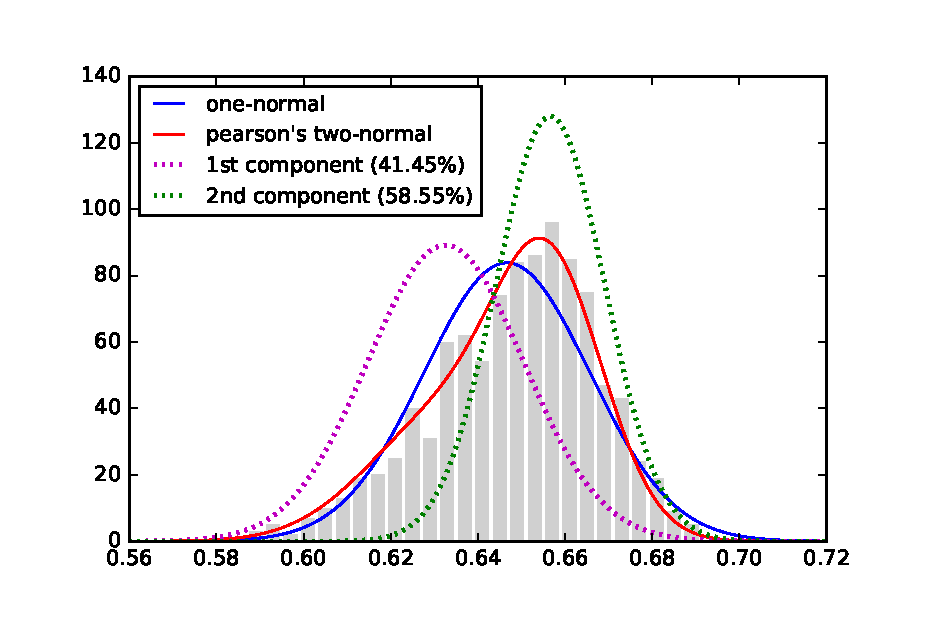
\includegraphics[width=0.8\linewidth]{figures/pearson-crab.eps}
  \caption{In this plot, the bar chart of the observations from Weldon is shown
    in grey. The blue solid line shows the single normal distribution fitting
    the data using Maximum Likelihood; And the solid line in red plots the
    mixture model of two normals distributions derived by Pearson using moment
    matching where its two components are also displayed in green and purple
    dotted lines.}
  \label{fig::pearson-crab}
  \end{subfigure}
  ~
  \begin{subfigure}[b]{0.95\textwidth}
  \centering
  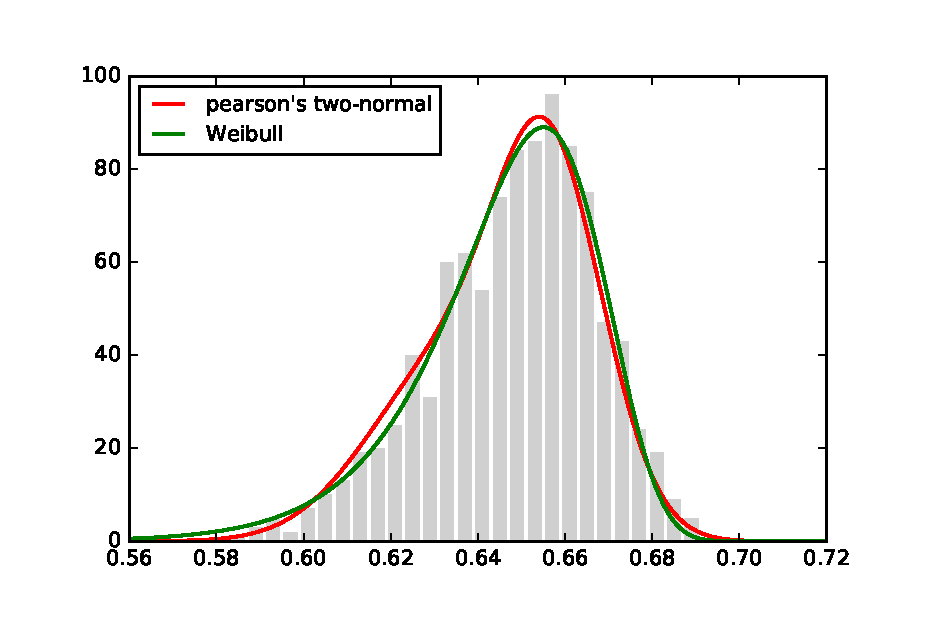
\includegraphics[width=0.8\linewidth]{figures/pearson-crab-weibull.eps}
  \caption{Comparison between the Pearson's mixture of two normals and a single
  Weibull distribution. Pearson's mixture model provides a better fitting at the
  mode of empirical distribution. Note that the form of density function of
  Weibull distribution is much more complicated than that of normal distribution
  and it requires numeric means to estimate the parameters.}
  \label{fig::pearson-crab-weibull}
  \end{subfigure}
  \caption{Pearson's Mixture of Two Normals on ``Breadth of Forehead of Crabs''}
\end{figure}

Pearson used two normal distributions to fit the observations. To estimate the
parameters, namely, the means ($\mu_1, \mu_2$) and standard-variance ($\sigma_1,
\sigma_2$) of the two normal distributions as well as the proportions ($\pi_1,
\pi_2$) of the two components, Pearson followed the method of moments (which
was also introduced by himself in 1894). Though moment matching is superseded
by Fisher's method of maximum likelihood~\cite{pfanzagl1994parametric} in
nowadays classic statistical modelling, it was a numerically simpler approach
in most cases. However, the calculation was still formidable and daunting at
the time without the aid of computer or other machinery of any kind.
Mathematically, the problem involves five parameters $\mu_1, \mu_2, \sigma_1,
\sigma_2$ and $\pi_1$ (we can obtain $\pi_2 = 1 - \pi_1$) and to find a
solution the parameters need to ensure that the mixture matches on the first
five moments. Pearson derived a ninth degree polynomial (nonic) and two
candidate real roots are found. He finally chose the solution on the basis of
agreement with the sixth moment. In Figure~\ref{fig::pearson-crab}, the dashed
curve in red shows Pearson's mixture and its two components are displayed in
purple and green dashed lines. Clearly, the mixture is skewed and better fits
the histogram. And indeed, two subspecies are identified which verifies the
hypothesis of Weldon.

It is quite an advanced idea to leverage latent variables for statistical
modeling at that time. Otherwise fitting the asymmetric observations would
involve a much more complicated distribution. In fact, we can also fit the data
with a skewed Weibull distribution, the parameter of which are nevertheless
computational difficult to estimate (The Maximum Likelihood estimator for the
shape parameter is the solution to the equation $\frac{1}{k} =
\frac{\sum_{i=1}^N (x_i^k\log x_i - x_N^k \log x_N) }{\sum_{i=1}^N (x_i^k -
x_N^k)}- \frac{1}{N}\sum\limits_{i=1}^N \log x_i$, and numeric methods, which
were very primitive at the time of late 19th century, is required.) Therefore
Weibull distribution was not a practical option for fitting the data without the
aid of computers. In Figure~\ref{fig::pearson-crab-weibull}, we compare the
Peason's mixture of two normals with one single Weibull distribution fitting the
data using Maximum Likelihood. The difference between the two curves is not
significant. However, Pearson's result seems to fit better at the mode around
$0.66$.

\subsection{Mixture Models --- Development of EM algorithm}

Although solving the mixture model with the method of moments is a very
laborious task and performing the necessary calculation is even more
heroic~\cite{mclachlan2004finite}, it does not always yield the optimal solution
in the statistical sense. The maximum likelihood approach, however, possesses
superior statistical property as it tries to place higher probability close to
the observed data and are more often unbiased. With the development of computer
and optimization in the last century, modern statistical modeling is able to
utilize numeric algorithms to solve Maximum Likelihood Estimator (MLE).  Among
the different optimization methods, Expectation-Maximization (EM)
algorithm~\cite{dempster1977maximum} has greatly stimulated interest in the use
of mixture models as well as other PLVMs. Several reasons can be accounted for
the popularisation of EM algorithm: (1) It is generally easy to implement the
algorithm and it has virtually no parameters to tune, as compared to, for
example, gradient descent, where a carefully selected learning step is required
to ensure fast training; (2) It usually does not need any special treatment to
handle the constraints of the model. For example, in the normal mixture problem,
the standard-variance of a component normal is always positive and in EM
algorithm and this is naturally satisfied since it is computed as the empirical
standard-variance of the ``generated'' completed data from the posterior
distribution; (3) EM is a flexible family of approaches where the variational
distribution in the expectation step can be simplified (or constrained) for the
purpose of computation efficiency (e.g. mean-field EM) and the maximization step
can also be substituted by an ascend step. We leave the details of EM algorithm
in Chapter~\ref{sec::bg-em}.  In this section, we provide a brief comparison
between EM algorithm and Pearson's method of moments and show how we can
improve Pearson's result by EM algorithm.

\begin{figure}[ht!]
  \centering
  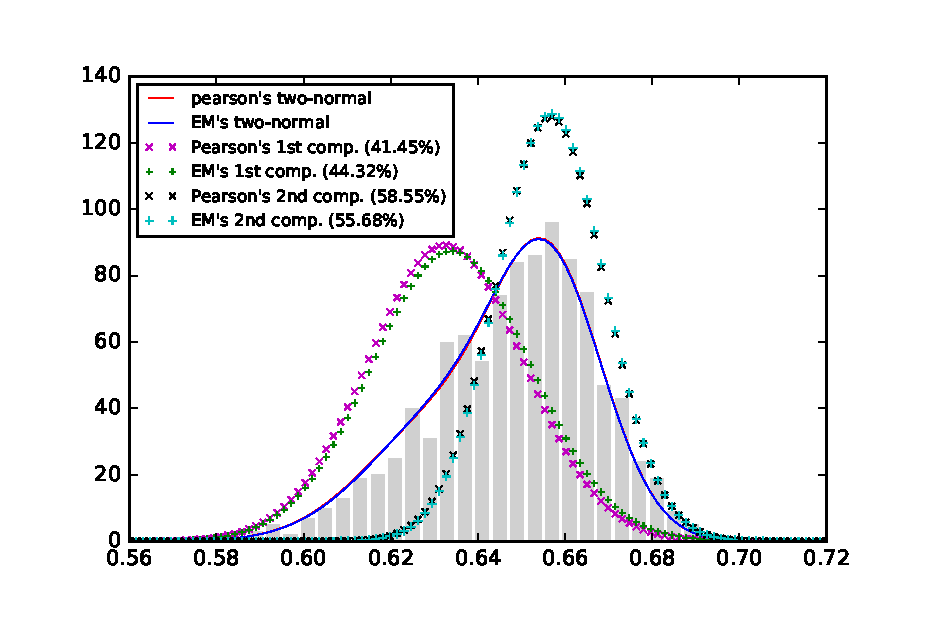
\includegraphics[width=0.8\linewidth]{figures/pearson-crab-em.eps}
  \caption{Comparison of the mixture model of two normals between Pearson's
  approach and EM algorithm. The two mixture models are very close to each
  other showing that the moment-matching method of Pearson obtains a near
  optimal likelihood.}
  \label{fig::pearson-crab-em}
\end{figure}

We plot the curves of the mixture models of the two methods as well as their
components in Figure~\ref{fig::pearson-crab-em}. The results are almost
identical. To assess the quality of the model quantitatively, Pearson used the
Chi-square test~\cite{pearson1900x} which he proposed to examine if the observed
data is indeed from the model. We follow his practice and report the result in
Table~\ref{tab::pearson-em-crab}.

\begin{table}[h]
  \centering
  \caption{Pearson's Chi-square test and p-Value for a single normal model, a
    single Weibull model, and the two normal mixture model of Pearson and EM
    algorithm in the ``Breadth of Forehead of Crabs'' problem. For the normal
    models, we also include the model parameters.}
  \label{tab::pearson-em-crab}
  \setlength\tabcolsep{5pt}
  \begin{tabular}{c|cccccc|c|cc}
    Method & $\mu_1$ & $\mu_2$ & $\sigma_1$ & $\sigma_2$ & $\pi_1$ & $\pi_2$
           & freedom & Chi-square & p value \\ \hline \hline
    Single Normal & 0.6466 & \NA & 0.0190 & \NA & 1 & \NA & 2 & 71.6836 &
    \num{2.157e-6} \\
    Single Weibull & \NA & \NA & \NA & \NA & \NA & \NA &
    2 & 28.3841 & 0.2904 \\
    Pearson & 0.6326 & 0.6566 & 0.0179 & 0.0125 & 0.4145 & 0.5855 &
    5 & 21.0342 & 0.5186 \\
    EM & 0.6339 & 0.6568 & 0.0182 & 0.0124 & 0.4432 & 0.5568 &
    5 & 20.8438 & 0.5304 \\
    %\hline \hline
  \end{tabular}
\end{table}

As expected, we see that the EM algorithm results in the smallest Pearson's
Chi-square. In less mathematical terms, the observed data is distributed more
close to the model given by the EM algorithm. In addition, the p-values in the
significant test show that it is more certain that the data is sampled from the
mixture normal of EM algorithm. To an extent, the assessment on the Weldon's
crab dataset justifies the use of EM algorithm to solve MLE in applications of
mixture modeling.

% EM:         (statistic=20.843800910788627, pvalue=0.53040874121547321)
% Pearson:    (statistic=21.034210586530026, pvalue=0.51862468978687204)
% uni-normal: (statistic=71.683615393997414, pvalue=2.1571531876646807e-06)
% Pearson:    (0.6326, 0.6566, 0.0179, 0.0125, 0.4145, 0.5855)
% EM:         (0.6339, 0.6568, 0.0182, 0.0124, 0.4432, 0.5568)
% Weibull:    (statistic=28.384054004025337, pvalue=0.29047889023764795)

\subsection{From Mixture Models to Topic Modeling}

Since the late of 1990s, the study on document understanding has witnessed a new
rising approach of PLVMs which is often referred as topic modeling. The first
well recognized topic modeling method, probabilistic latent semantic
indexing~(PLSI)~\cite{hofmann1999probabilistic}, is simple yet effective.
Essentially it sees the distribution $w_d$ of unigrams for a document $d$ as a
$K$-mixture of multinomial distributions $\beta_1, \dots, \beta_K$ with
proportions $\theta_{d, 1}, \dots, \theta_{d, k}$. Those $\beta_K$ are referred
as ``topics'' because the words of large probabilities in a component are often
semantically related. In addition, the topic weights $\theta_d$ of a document
provides a short summary of the documents.  Computationally, $\theta_d$ has a
much lower dimensionality than $w_d$ and thus can be leveraged as a (part of)
feature vector in tasks such as document classification or clustering. Moreover,
$\theta_d$ is semantically meaningful as similarity of $\theta_d$ correlates
with the subject of the documents, which can be greatly useful in document
understanding.

Later development of topic modeling includes numerous works which are beyond of
the focus in this thesis. In terms of modeling the latent variables, there are
two aspects of milestone progress that are worth a brief overview: the Bayesian
inference and nonparametric statistics. The early effort promoting the Bayesian
nonparametrics and advocating the theoretical formalization of topic modeling,
specifically, the analysis on random processes of exchangeable
partitions~\cite{pitman1995exchangeable}, are the lectures taught by
\citeauthor{pitman2002combinatorial} at Berkeley in Spring
\citeyear{pitman2002combinatorial}. Many of David Blei's later
works~\cite{blei2009topic,blei2003latent,blei2010nested} are immediate fruit of
the lectures and readers interested in a principle introduction on this topic
should refer to the lecture notes~\cite{pitman2002combinatorial} and the
references therein.

\emph{Bayesian inference} departs from the tradition MLE framework. It assumes a
prior distribution on latent variables parametrized by the
\emph{hyperparameters}. The advantages of introducing a prior on latent
variables are mainly two folds and we show them using the Latent Dirichlet
Allocation~(LDA)~\cite{blei2003latent} as an example: (1) It enables user to
incorporate human knowledge about the latent variables into modeling. In
document understanding, the word distribution of a topic as well as the
proportion of topics for a document are naturally sparse. LDA encourages such
behavior by adding a Dirichlet prior. (2) By selecting the form of prior
carefully, the prior and posterior can be in the same (with different parameters
though). Such conjugate prior-posterior pairs are computational beneficial in
both Gibbs sampling as well as variational inference. LDA chooses Dirichlet as
the conjugate prior to multinomial distribution. Another significant difference
between Bayesian inference and MLE is the estimation method. There are two major
estimation methods of the latent variables in Bayesian setting which are
Bayesian estimator (posterior expectation) and maximum a posterior (MAP). The
first computes the posterior expectation of the latent variables given the
observed data while the second selects the value with the maximal probability in
the posterior distribution, which can be viewed as an extension of the MLE
method. In the context of topic modeling, it has been noticed that Bayesian
estimator is more popular than the alternatives. The major criticism of MAP is
the fact that it is not very representative of Bayesian methods in general
because it is still a point estimates in nature. Specifically in topic modeling,
it is common that the posterior distribution of the latent variables are in fact
multi-modal and therefore it is computational infeasible (or even intractable)
to calculate MAP due to the non-convex nature of the problem.

\emph{Nonparametric statistics} aims to model the data with possibly infinite
number of latent variables. In topic modeling, it means that one can model
infinite large number of topics or words in the vocabulary. Although in practice
it does not seem to be useful immediately since there is always a finite
upper-bound for these quantities, it relies on expert knowledge to appropriately
select the values. Nonparametric statistics are most powerful to learn the
number of latent variables that are adequately large to explain the data by
using random processes. Random processes are extensively studied in recent
literature, as surveyed in \cite{hajek2015random}, including Gaussian
process~\cite{rasmussen2006gaussian}, Dirichlet process~\cite{teh2011dirichlet},
Indian buffet process~\cite{ghahramani2005infinite}, and hierarchical
processes~\cite{teh2012hierarchical,griffiths2004hierarchical,blei2010nested},
just to name a few. Mathematically, to model the latent variables from possibly
infinite number of choices, the nonparametric approach assumes a random process
as prior. Computationally, there are mainly two strategies, Gibbs sampling and
truncated variational inference, to estimate the posterior distribution of the
possibly infinite number of latent variables. Gibbs sampling takes advantage of
the fact that the prior process usually yields a simple prediction rule of one
latent variable given all others. For example, in Dirichlet process, using the
notion of Chinese restaurant process~\cite{pitman2002combinatorial}, the
probability of a latent variable choosing an existing or a new value is
proportional to the sum of a hyperparameter $\alpha$ and the number of other
latent variables of the same value:

\begin{eqnarray}
  \P_{CRP}(z_i = k | z_1, \dots, z_{i-1}, z_{i+1}, \dots, z_N)
    \propto
      \begin{cases}
        \alpha + \sum\limits_{j = 1, j \neq i}^N \indct( z_j = k )
        & \text{if $k < K$} \\
        \alpha
        & \text{if $k = K + 1$}
      \end{cases} \\
\end{eqnarray}
Where it is supposed that the value of $z_j, j \neq i$ is choosing from $1,
\dots, K$  and for any $k < K$ the support is nonempty. Therefore it is feasible
to investigate sampling methods for inference. While alternatively, another
strategy for estimation is to approximate the possibly infinite posterior with a
finite approximation. For the Dirichlet Process (as well as the generalized
Pitman-Yor two-parameter process~\cite{pitman1997two}), the truncating
approximation is based on a stick-breaking~\cite{ishwaran2011gibbs}
interpretation. It views the process as breaking a stick with the proportion as
a sample from a Beta distribution and the truncation stops the breaking after
there is a predefined number of sticks generated. Both of the above two
strategies have advantages as Gibbs sampling does not need to truncate the size
of latent variables by a finite number while the truncated variational inference
is generally more computational efficient. However, as shown in
\cite{wang2012truncation}, it is possible to combine the two ideas together by
performing the E-step in the variational EM via sampling.

\section{Latent Variable for Optimization}

Previous research such as topic modeling mainly incorporates the latent
variables for the purpose of knowledge discovery. Another motivation to use
latent variable models is efficient computation. In previous discussion, we have
already witnessed that by introducing latent variable, the mixture model of
Pearson is much more easier to compute than that of Weibull distribution.
However, contemporary effort in the direction of leveraging PLVMs for efficient
computation was less explored. In one of the recent work by the author,
Dual-Clustering Maximum Entropy (DCME)~\cite{wang2016dcme}, it demonstrats that
the PLVM is an effective means to improve the optimization efficiency.

Maximum Entropy is an classic approach in classification as well as word
embedding. However, it becomes computationally challenging when the number of
classes or the vocabulary size is large. DCME approaches the problem by
optimizing ME in its primal-dual form. The key insight is to introduce a latent
cluster assignment for each training instance and assume that the dual variables
of an instance are determined by the corresponding latent assignment. As an
initial investigation, we use the latent variables in a much simpler manner than
the mixture models. Specifically, we restrict the latent variable distributed as
a Kronecker delta which has support only on a single value, as contrast to the
case of mixture model where the latent variable is distributed as a more general
multinomial. DCME naturally leads to an approximation of the dual variables
which can be computed by a K-means like clustering. In addition, it also enables
a efficient online-offline computation scheme whose computation complexity does
not depends on the number of classes nor the vocabulary size. And the empirical
study demonstrated that DCME outperforms other state-of-the-art approaches.

\section{Overview of This Thesis}

In the rest of this thesis, we will discuss in detail on the PLVMs.
Specifically,  In chapter~\ref{chp::bg}, we briefly discuss a few key
mathematics that can greatly facilitate the understanding of the PLVMs.

Next, we will show two scenarios where PLVMs are applied in data mining for
knowledge discover.

The first work analyzes the citations of
literatures~\cite{wang2013understanding}. Understanding how research themes
evolve over time in a research community is useful in many ways (e.g., revealing
important milestones and discovering emerging major research trends).  In this
study, we propose a novel way of analyzing literature citation to explore the
research topics and the theme evolution by modeling article citation relations
with a probabilistic generative model.  The key idea is to represent a research
paper by a ``bag of citations'' and model such a ``citation document'' with a
probabilistic topic model.  We explore the extension of a particular topic
model, i.e., Latent Dirichlet Allocation~(LDA), for citation analysis, and show
that such a Citation-LDA can facilitate discovering of individual research
topics as well as the theme evolution from multiple related topics, both of
which in turn lead to the construction of evolution graphs for characterizing
research themes.  We test the proposed citation-LDA on two datasets: the ACL
Anthology Network~(AAN) of natural language research literatures and PubMed
Central~(PMC) archive of biomedical and life sciences literatures, and
demonstrate that Citation-LDA can effectively discover the evolution of research
themes, with better formed topics than (conventional) Content-LDA.

The second work explores PLVMs in a crowdsourcing setting~\cite{wang2016tpp}.
Crowdsourcing services make it possible to collect huge amount of annotations
from less trained crowd workers in an inexpensive and efficient manner.
However, unlike making binary or pairwise judgements, labeling complex
structures such as ranked lists by crowd workers is subject to large variance
and low efficiency, mainly due to the huge labeling space and the annotators'
non-expert nature. Yet ranked lists offer the most informative knowledge for
training and testing in various data mining and information retrieval tasks such
as \textit{learning to rank}.  In this paper, we propose a novel generative
model called ``Thurstonian Pairwise Preference'' (\textsc{Tpp}) to infer the
true ranked list out of a collection of crowdsourced pairwise annotations.  The
key challenges that \textsc{Tpp} addresses are to resolve the inevitable
incompleteness and inconsistency of judgements, as well as to model variable
query difficulty and different labeling quality resulting from workers' domain
expertise and truthfulness.  Experimental results on both synthetic and
real-world datasets demonstrate that \textsc{Tpp} can effectively bind pairwise
preferences of the crowd into rankings and substantially outperforms previously
published methods.

In addition, as hinted before, another aspect of PLVMs is to improve the
efficiency of optimization. To this end, we devote another chapter to discuss
the study of Dual-Clustering Maximum Entropy~\cite{wang2016dcme}.  Maximum
Entropy (ME), as a general-purpose machine learning model, has been successfully
applied to various fields such as text mining and natural language processing.
It has been used as a classification technique and recently also applied to
learn word embedding. ME establishes a distribution of the exponential form over
items (classes/words). When training such a model, learning efficiency is
guaranteed by \emph{globally} updating the entire set of model parameters
associated with \emph{all} items at \emph{each} training instance. This creates
a significant computational challenge when the number of items is large. To
achieve learning efficiency with affordable computational cost, we propose an
approach named Dual-Clustering Maximum Entropy (DCME).  Exploiting the
primal-dual form of ME, it conducts clustering in the dual space and
approximates each dual distribution by the corresponding cluster center.  This
naturally enables a hybrid online-offline optimization algorithm whose time
complexity per instance only scales as the product of the feature/word vector
dimensionality and the cluster number. Experimental studies on text
classification and word embedding learning demonstrate that DCME effectively
strikes a balance between training speed and model quality, substantially
outperforming state-of-the-art methods.


\include{2-related}
\include{3-model}
\include{4-predictions}

\chapter{Conclusions}

We conclude that graduate students like coffee.
% \iffalse
%<example>
% \fi
% \end{verbatim} \hrule \end{quote}
%
% \subsection{Reference Matter}
%
% \DescribeMacro{\appendix}
% To switch from the body of your thesis to the reference material
% at the end, you should use the standard \LaTeX\ |\appendix| command.
% In \pkg{uiucthesis2009}, there is also a starred version of this command
% that eliminates the lettering of the appendices (use if you have
% a single appendix). Note that if you use |\appendix*| along with
% the |[fancy]| option, you may want to put ``Appendix:'' at
% the beginning of the chapter title.
%
%
% \begin{quote} \hrule \begin{verbatim}
\appendix*

\include{Appendix.tex}
% \end{verbatim} \hrule \end{quote}
% \iffalse
%<example>
% \fi
%
% \subsection{Back Matter}
%
% \DescribeMacro{\backmatter}
% The last few chapters in your thesis should not have chapter
% numbers, but should be listed in the Table of Contents.
% These chapters include the Bibliography, the Index,
% and the Vita.  \LaTeX's |\backmatter| command accomplishes this.
%
% \DescribeMacro{\bibliography}
% Use the standard \LaTeX\ bibliography commands to
% create your bibliography. Most people will use Bib\TeX\ to do this.
% (See \cite{Lamport}). For those in the sciences, you may want to
% check out the \pkg{cite} package (it's pretty standard), which
% will produce numerical citations that are sorted and compressed.
% You can also use the \pkg{natbib} package. Both of these packages
% can do either bracketed citations or superscript citations.
%
% \DescribeMacro{\vita}
% The |\vita| command begins a new chapter for your vita.
% In fact, it does exactly the same thing as |\chapter{\vitaname}|,
% where |\vitaname| is ``Vita.''
%
% \begin{quote} \hrule \begin{verbatim}
\backmatter

\bibliography{thesisbib}

\chapter{Vita}

Juan Valdez was born\ldots.

\end{document}
% \end{verbatim} \hrule \end{quote}
%
% \iffalse
%</example>
% \fi
%
% \section{User Customization}
%
% \DescribeMacro{\draftheader}
% If you don't like the header that the the |[draftthesis]| option
% creates, you can redefine the |\draftheader| command so that it
% produces whatever text you want.
%
% \DescribeMacro{\thesisspacing}
% The \pkg{uiucthesis2009} class loads \pkg{setspace} for the
% line spacing commands.  See the documentation in that package
% for more information on the commands it provides.
% By default, \pkg{uiucthesis2009} uses one and a half line spacing,
% or double spacing if the |[fullpage]| option is specified.
% If you're unhappy with that, you can override it by redefining the
% |\thesisspacing| command.
%
% \DescribeMacro{\nocopyrightpage}
% Unless the |[draftthesis]| option is used, a page with the copyright notice
% is printed before the title page. If you don't want this page to
% appear, even in the final version, put the |\nocopyrightpage| macro
% somewhere in the preamble.
%
% \DescribeMacro{\toclabels}
% Some departments require the Table of Contents, List of Tables and
% List of Figures to have a ``Page'' heading over the page numbers
% on the first page. This can be accomplished by putting the |\toclabels|
% command somewhere before the |\tableofcontents| command. (NOTE: if you put
% the |\tableofcontents| command in a separate file that you |\include| in
% the main file, the |\toclabels| command must also be in that file.)
%
% \DescribeMacro{\chaptertitlefont}
% \DescribeMacro{\sectiontitlefont}
% \DescribeMacro{\subsectiontitlefont}
% \DescribeMacro{\subsubsectiontitlefont}
% These macros contain the font declarations for the corresponding sectioning
% levels and can be redefined to suit your aesthetic desires. Use
% |\renewcommand| to do this in the preamble.
%
% \DescribeMacro{\chapternumberfont}
% The |\chapternumberfont| macro is really most applicable when the |[fancy]| option is used. It
% specifies the font declaration used for the chapter number set in the left
% margin next to the title. Otherwise it specifies the font used to print
% the words ``Chapter \#'' at the top of each chapter's opening page. Use
% |\renewcommand| to redefine this macro in the preamble.
%
% \DescribeMacro{\chaptertitleheight}
% |\chaptertitleheight| is the amount of space allotted for the chapter title at the top
% of the page. You can redefine it using |\setlength| in the preamble.
%
% \DescribeMacro{\bibname}
% |\bibname| is a standard \LaTeX\ macro that contains the title of the reference
% section at the end of your thesis; ``References'' by default. Use
% |\renewcommand| to redefine it in the preamble.
%
% \DescribeMacro{\vitaname}
% Like |\bibname| but it contains the name used for your vita at the very end.
% The Grad College allows ``Vita'', ``Author's Biography'', or ``Curriculum Vitae'',
% each of which is slightly different in format.  See \cite{Handbook}.
%
% \DescribeMacro{\abstractname}
% Like above, but for the abstract. By default, ``Abstract''.
%
% \DescribeMacro{other "name"s}
% Similarly, the titles for the Table of Contents, List of Figures, and List of Tables
% are stored in the macros |\contentsname|, |\listfigurename|, and |\listtablename|,
% respectively. Their default values are the names in the previous sentence. There are
% also the macros |\chaptername|, |\appendixname|, |\indexname|, |\partname|,
% |\tablename|, and |\figurename| that contain the appellations for chapter and appendix
% headings (not applicable with the |[fancy]| option), the index, parts, tables, and figures.
% Their default values are Chapter, Appendix, Index, Part, Table, and Figure, respectively.
% All of these macros can
% be redefined in the preamble with |\renewcommand|.  These macros are all part of
% the standard \LaTeX\ formalism, they are just included here for the reader's convenience.
% For example, some departments require chapter headings to be in all caps, which can
% be done by changing the |\chaptername| macro to be CHAPTER.
%
% \DescribeMacro{\note}
% This command inserts a marginal note just like |\marginpar| with two distinctions:
% First, the note is single-spaced in a smaller type for compactness.
% Second, it is only printed when
% the |[draftthesis]| option is used. Since marginal notes are not allowed in the final
% draft, the |\note| command is recommended over the |\marginpar| command.
%
% \section{Backwards Compatibility}
%
% Compatibility with previous versions of \pkg{uiucthesis2009} are supported. Previously it
% was implemented as a package rather than a class, in which case you opened the document
% with:
% \begin{quote} \hrule \begin{verbatim}
% \documentclass[oneside,...]{book}
% \usepackage[...]{uiucthesis2009}
% \end{verbatim} \hrule \end{quote}
% To provide backwards-compatibility, a style file is provided that has the same functionality
% of the class file described herein. Similarly, (really) old versions of \pkg{uiucthesis2009}
% used the \env{preliminary} and \env{thesis} environments, which are now deprecated
% but backwards-compatibility support is still provided.
%
% \section{Other Issues}
%
% \subsection{Paper Size and PDF Files}
%
% The default paper size for most \LaTeX\ distributions is A4, which is slightly different
% the 8.5 x 11 size for letter paper in the U.S\@. The Graduate College requires theses
% to be letter paper size.  In addition, many departments want soft copies of the thesis
% in PDF format. Unfortunately, the program used to convert the dvi file to PDF format
% (|dvipdfm| on my computer, which is a Windows machine with Mik\TeX installed on it)
% often produces PDF files in A4 format, even if |letterpaper|
% is specifically specified in the your \TeX source file. If you're having this problem,
% either run the PDF conversion utility from the command line with the right flag ---
% for example, |dvipdfm -p letter| on my computer --- or change the default paper size in
% the config file for your PDF conversion utility, which will then fix this problem
% permanently.  On my computer, this can be done by going to the |dvipdfm\config|
% subdirectory off of the main \TeX installation directory (usually |C:\texmf|). In this
% directory is a file called |config| that has a line for the default paper size.
%
% \subsection{Reference Lists at the Chapter Level}
%
% The \pkg{cite} package includes a style file \pkg{chapterbib.sty} that can be used
% to do a list of references for each chapter instead of just one big list at the
% end of the thesis.  I've not used this style before so you're on your own if you
% want to do this, but I think it is rather straightforward\ldots.
%
% \StopEventually{%
%   \begin{thebibliography}{9}
%     \bibitem{Handbook}
%     \emph{Handbook for Graduate Students Preparing to Deposit}.
%     \newblock Graduate College, University of Illinois at
%     Urbana-Champaign, 2004
%
%     \bibitem{thesisweb}
%      \emph{Grad College webpage with thesis requirements}.
%      \newblock |http://www.grad.illinois.edu/graduate-college-thesis-requirements|
%
%     \bibitem{Lamport}
%     Leslie Lamport.
%     \newblock \emph{\LaTeX: A Document Preparation System}.
%     \newblock Addison-Wesley, 1994.
%   \end{thebibliography}
% }
%
% \section{Implementation}
%
% This section shows the implementation of the \pkg{uiucthesis2009} class.
% Unless you are interested in the details of how \pkg{uiucthesis2009} works,
% you probably don't need to read it.
%
% \iffalse
%<*class|package>
\RequirePackage{setspace}
% \fi
%
% \subsection{Compatibility}
%
% Provide compatibililty with older versions of \LaTeX.
% \begin{macro}{\@ifundefined}
%    \begin{macrocode}
\expandafter\ifx\csname @ifundefined\endcsname\relax
  \def\@ifundefined#1{%
    \expandafter\ifx\csname#1\endcsname\relax
      \expandafter\@firstoftwo
    \else
      \expandafter\@secondoftwo
    \fi}
\fi
%    \end{macrocode}
% \end{macro}
%
% \begin{macro}{\MakeUppercase}
%    \begin{macrocode}
\@ifundefined{MakeUppercase}{\let\MakeUppercase=\uppercase}{}
%    \end{macrocode}
% \end{macro}
%
% \subsection{Option Processing}
%
%    \begin{macrocode}
\newif\if@thesisdraft \@thesisdraftfalse
\newif\if@thesisfancy \@thesisfancyfalse
\newif\if@fullpage \@fullpagefalse
\newif\if@largecaps \@largecapsfalse
\newif\if@proquest \@proquestfalse
\newif\if@edeposit \@edepositfalse
\newif\if@thesisoffcenter \@thesisoffcenterfalse
\newif\if@centerchapter \@centerchapterfalse
%    \end{macrocode}
%
%    \begin{macrocode}
\DeclareOption{draftthesis}{\@thesisdrafttrue}
\DeclareOption{fancy}{\@thesisfancytrue}
\DeclareOption{fullpage}{\@fullpagetrue}
\DeclareOption{proquest}{\@proquesttrue}
\DeclareOption{toclabels}{\AtBeginDocument{\toclabels}}
\DeclareOption{edeposit}{\@edeposittrue}
\DeclareOption{offcenter}{\@thesisoffcentertrue}
\DeclareOption{centerchapter}{\@centerchaptertrue}
%    \end{macrocode}
%
% The |[largecaps]| option causes the title and author's name to
% be use a ``large caps'' font on the title page.  Otherwise,
% \pkg{uiucthesis2009} just converts them to uppercase and uses the
% normal fonts.  The difference is that the spacing between the
% characters in the large caps font is tuned for setting type in all caps.
%
% The large caps font is \emph{not a standard font}, and so it will not exist
% unless you have installed it.
%
%    \begin{macrocode}
\DeclareOption{largecaps}{\@largecapstrue}
%    \end{macrocode}
%
% Load the \pkg{book} class with the |[oneside]| and |[letterpaper]| options
%
%    \begin{macrocode}
%<class>\DeclareOption*{\PassOptionsToClass{\CurrentOption}{book}}
%<class>\PassOptionsToClass{letterpaper,oneside}{book}
\ProcessOptions
%<class>\LoadClass{book}
%    \end{macrocode}
%
% If the |[proquest]| option is used, turn off output to auxiliary files so
% that the thesis doesn't have to be recompiled again to get all the references
% correct. Also double-space the ProQuest abstract and use the full page.
%
%    \begin{macrocode}
\if@proquest
    \nofiles    % don't overwrite the .aux files
    \def\makeindex{}
    \@thesisfancyfalse
    \@fullpagetrue
\fi
%    \end{macrocode}
%
% If the |[draftthesis]| option was specified, define the |\draftheader| macro.
%
%    \begin{macrocode}
\if@thesisdraft
  \newcount\timehh\newcount\timemm
  \timehh=\time \divide\timehh by 60
  \timemm=\time \count255=\timehh \multiply\count255 by -60
    \advance\timemm by \count255
  \def\draftheader{\slshape Draft of \today\ at
  \ifnum\timehh<10 0\fi\number\timehh\,:\,\ifnum\timemm<10 0\fi\number\timemm}%
\fi
%    \end{macrocode}
%
% Define the |\toclabels| command which prints the headings in the Table of Contents,
% List of Figures and List of Tables.
%
%    \begin{macrocode}
\newcommand{\toclabels}{%
    \addtocontents{toc}{\vspace*{-\baselineskip}\hfill Page\endgraf}%
    \addtocontents{lof}{\vspace*{-\baselineskip}~Figure\hfill Page\endgraf}%
    \addtocontents{lot}{\vspace*{-\baselineskip}~Table\hfill Page\endgraf}}
%    \end{macrocode}
%
% \subsection{Title Page}
%
% \begin{macro}{\title}
% \begin{macro}{\author}
% Override the standard definitions of |\title| and |\author| to also
% define uppercased versions.
%    \begin{macrocode}
\def\@mkuptitle#1{\gdef\@Utitle{#1}}
\def\title#1{\gdef\@title{#1}\MakeUppercase{\protect\@mkuptitle{#1}}}
\def\@mkupauthor#1{\gdef\@Uauthor{#1}}
\def\author#1{\gdef\@author{#1}\MakeUppercase{\protect\@mkupauthor{#1}}}
%    \end{macrocode}
% \end{macro}
% \end{macro}
%
% \begin{macro}{\phdthesis}
% \begin{macro}{\msthesis}
% \begin{macro}{\otherdoctorate}
% \begin{macro}{\othermasters}
% \begin{macro}{\department}
% \begin{macro}{\college}
% \begin{macro}{\schools}
% \begin{macro}{\degreeyear}
% \begin{macro}{\committee}
% \begin{macro}{\volume}
% Macros to set title page elements.
%    \begin{macrocode}
\def\phdthesis{\def\@degree{Doctor of Philosophy}
    \def\degree{Ph.D.}
    \def\@thesisname{DISSERTATION}
    \def\@committeename{Doctoral Committee:}
    }
\def\msthesis{\def\@degree{Master of Science}
    \def\degree{M.S.}
    \def\@thesisname{THESIS}
    \def\@committeename{Master's Committee:}
    }
\newcommand{\otherdoctorate}[2]{\def\@degree{#1}
    \def\degree{#2}
    \def\@thesisname{DISSERTATION}
    \def\@committeename{Doctoral Committee:}
    }
\newcommand{\othermasters}[2]{\def\@degree{#1}
    \def\degree{#2}
    \def\@thesisname{THESIS}
    \def\@committeename{Master's Committee:}
    }
\def\department#1{\def\@dept{#1}}
\def\college#1{\def\@college{#1}}
\def\schools#1{\def\@schools{#1}}
\def\degreeyear#1{\def\@degreeyear{#1}}
\newcommand{\committee}[1]{\gdef\@committee{#1}}
\newcommand*{\volume}[1]{\gdef\thesis@volume{VOLUME~#1}}
\newcommand*{\thesis@volume}{}
\if@edeposit
  \gdef\@committee{%
%<class>    \ClassError{uiucthesis2009}{A committee must be specified for e-deposit dissertations.}%
%<package>    \PackageError{uiucthesis2009}{A committee must be specified for e-deposit dissertations.}%
    {Use \protect\committee\space with members separated by \protect\\'s.}}
\fi
%    \end{macrocode}
% \end{macro}
% \end{macro}
% \end{macro}
% \end{macro}
% \end{macro}
% \end{macro}
% \end{macro}
% \end{macro}
% \end{macro}
% \end{macro}
%
% \begin{macro}{\copyrightnotice}
% Define the copyright notice as a macro so that the user
% can change it if desired.
%    \begin{macrocode}
\def\copyrightnotice{\copyright~\@degreeyear~by \@author. All rights reserved.}
%    \end{macrocode}
% \end{macro}
% \begin{macro}{\nocopyrightpage}
% The printing of the copyright page can also be turned off with the
% |\nocopyrightpage| command (must come before |\maketitle|):
%    \begin{macrocode}
\newif\if@thesiscrpage \@thesiscrpagetrue
\let\nocopyrightpage\@thesiscrpagefalse
\if@thesisdraft\nocopyrightpage\fi
%    \end{macrocode}
% \end{macro}
%
% Set the default title page elements.
%    \begin{macrocode}
\phdthesis
\department{Computer Science}
\college{Graduate College}
\def\@schools{}
\def\@degreeyear{\number\year}
%    \end{macrocode}
%
%
% \begin{macro}{\maketitle}
% Redefine \pkg{book}'s |\maketitle| command to produce
% the titlepage in the correct format.
%
%    \begin{macrocode}
\renewcommand\maketitle{
%    \end{macrocode}
% Print the copyright page if we're supposed to.
%    \begin{macrocode}
    \if@thesiscrpage
        \newpage
        \thispagestyle{empty}
        \null\vfill
        \centerline{\copyrightnotice}%
        \vskip 3ex % skip to visually center copyright notice
        \vfill
    \fi
%    \end{macrocode}
% Now start a new page for the title page.  It is single-spaced.
%    \begin{macrocode}
    \newpage
    \thispagestyle{empty}%
    \enlargethispage{1in}%
    \begingroup
    \def\baselinestretch{1}
%    \end{macrocode}
% Check what size font we are using for the text and select a
% smaller size appropriately.
%    \begin{macrocode}
    \ifnum \@ptsize=2
        \@normalsize
        \newcommand{\thesis@small}{\small}
    \else
        \large
        \newcommand{\thesis@small}{\@normalsize}
    \fi
%    \end{macrocode}
% We have to be careful to get the vertical position right.  The
% easiest way to do this seems to be to just set |\topmargin|,
% |\headheight|, and |\headsep| for this page.
%    \begin{macrocode}
    \headheight=0pt \headsep=0pt
    \topmargin=0in
%    \end{macrocode}
% Adjust the horizontal spacing so that the title page
% is centered on the page even if the rest of the document isn't.
% I'm not sure when |\textwidth| changes take place, so instead
% we calculate the correct |\oddsidemargin| to center the text column.
%    \begin{macrocode}
    \@tempdima=\paperwidth
    \advance\@tempdima by -\textwidth
    \divide\@tempdima by 2
    \advance\@tempdima by -1in
    \oddsidemargin=\@tempdima
    \let\evensidemargin=\oddsidemargin

%    \end{macrocode}
% Create the title page. Different spacing is used depending on whether the
% |[edeposit]| option is specified. Include the committee and the paragraph
% at the bottom of the page for e-deposit theses, as required by the Grad College.
%    \begin{macrocode}
    \newdimen\thesis@dim
    \if@edeposit
        \thesis@dim=1.5in
    \else
        \thesis@dim=1.5in
    \fi
    \newdimen\ct@dim
    \newdimen\cn@dim
    \ct@dim=\oddsidemargin
    \advance\ct@dim by -0.3125in
    \cn@dim=\oddsidemargin
    \advance\cn@dim by -0.6875in
    \if@largecaps
        \def\lc@selectfont{\fontshape{lc}\selectfont}%
    \else
        \def\lc@selectfont{}%
    \fi
    \begin{center}
    \if@edeposit
        \vbox to 1in{}
    \else
        \vbox to 1in{}
    \fi
    \vbox to \thesis@dim{%
        {\lc@selectfont\@Utitle}
        \if@thesisdraft
        \\[12pt]
        \draftheader
        \fi
        \vfil}%
    \vbox to 1.5in{%
        {\lc@selectfont BY}\\[12pt]
        {\lc@selectfont\@Uauthor}\\[12pt]
        \vfil}%
    \vbox to 0.5in{\thesis@volume\vfil}
    \vbox to 2.0in{%
        {\lc@selectfont \@thesisname}\\[12pt]
        Submitted in partial fulfillment of the requirements\\
        for the degree of \@degree\ in \@dept\\
        in the \@college\ of the\\
        University of Illinois at Urbana-Champaign, \@degreeyear\vfil}
	 \vskip -2ex
	 \vbox to 0.35in{
	 Urbana, Illinois}
	 \end{center}
	\begin{flushleft}
        \vbox to 0.3in{
        \hspace{-\ct@dim}\@committeename\\}
        \hspace{-\cn@dim}\begin{tabular}{l}\@committee\end{tabular}\vfil
	\end{flushleft}
    \newpage
    \endgroup
}
%    \end{macrocode}
% \end{macro}
%
% \subsection{Front Matter}
%
% \begin{macro}{\frontmatter}
% Redefine |\frontmatter| so that it sets the page number to 2 or 3, depending on whether or
% not the |[edeposit]| option is given.
%    \begin{macrocode}
\let\thesis@frontmatter=\frontmatter
\def\frontmatter{%
    \thesis@frontmatter
    \if@edeposit
        \setcounter{page}{2}
    \else
        \setcounter{page}{3}
    \fi}
%    \end{macrocode}
% \end{macro}
%
% \subsection{Table of Contents}
%
% \begin{macro}{\contentsname}
% Use ``Table of Contents'' instead of ``Contents''.
%    \begin{macrocode}
\renewcommand\contentsname{Table of Contents}
%    \end{macrocode}
% \end{macro}
%
% \begin{macro}{\l@chapter}
%    This code is a modified version of the code in the 1996/05/26 release
%    of classes.dtx that produces leader dots between the chapter
%    name and the page number.
%
%    This macro formats the entries in the table of contents for
%    chapters. It is very similar to |\l@part|
%
%    First we make sure that if a pagebreak should occur, it occurs
%    \emph{before} this entry. Also a little whitespace is added and a
%    group begun to keep changes local.
%    \begin{macrocode}
\renewcommand*\l@chapter[2]{%
  \ifnum \c@tocdepth >\m@ne
    \addpenalty{-\@highpenalty}%
    \vskip 1.0em \@plus 0.2em \@minus 0.2em
%    \end{macrocode}
%
%    The macro |\numberline| requires that the width of the box that
%    holds the part number is stored in \LaTeX's scratch register
%    |\@tempdima|. Therefore we put it there. We begin a group, and
%    change some of the paragraph parameters.  These are different
%    from the defaults for the standard report or book class.
%    \begin{macrocode}
    \setlength\@tempdima{1.5em}
    \begingroup
      \leftskip \z@ \rightskip \@tocrmarg \parfillskip -\rightskip
      \parindent \z@
%    \end{macrocode}
%    Then we leave vertical mode and switch to a bold font.
%    \begin{macrocode}
      \leavevmode \bfseries
%    \end{macrocode}
%    Because we do not use |\numberline| here, we have do some fine
%    tuning `by hand', before we can set the entry. We discourage but
%    not disallow a pagebreak immediately after a chapter entry.
%    We use leaders between the chapter title and the page number,
%    unlike the standard report or book class.
%    \begin{macrocode}
      \advance\leftskip\@tempdima
      \hskip -\leftskip
      #1\nobreak
      \leaders\hbox{$\m@th\mkern\@dotsep mu\hbox{.}\mkern\@dotsep mu$}
      \hfil \nobreak\hbox to\@pnumwidth{\hss #2}\par
      \penalty\@highpenalty
    \endgroup
  \fi}
%    \end{macrocode}
% \end{macro}
%
% \begin{macro}{\tableofcontents}
% We want the Table of Contents to be single-spaced, so
% we save the original definition, and then arrange it so
% that the new |\tableofcontents| calls |\singlespacing| before calling
% the original definition. Then set the flag mentioned above.
%    \begin{macrocode}
\let\thesis@tableofcontents=\tableofcontents
\def\tableofcontents{{\singlespacing\thesis@tableofcontents}}
%    \end{macrocode}
% \end{macro}
%
% \begin{macro}{\listoftables}
% \begin{macro}{\listoffigures}
% Similarly, redefine |\listoftables| and |\listoffigures| so
% that they use single spacing.
%    \begin{macrocode}
\let\thesis@listoftables=\listoftables
\def\listoftables{\newpage%
    \addcontentsline{toc}{chapter}{\listtablename}%
    {\singlespacing\thesis@listoftables}}
\let\thesis@listoffigures=\listoffigures
\def\listoffigures{\newpage%
    \addcontentsline{toc}{chapter}{\listfigurename}%
    {\singlespacing\thesis@listoffigures}}
%    \end{macrocode}
% \end{macro}
% \end{macro}
%
% \subsection{Other Frontmatter}
%
% \begin{environment}{abstract}
% The \env{abstract} environment is special because its contents are also
% used for the ProQuest abstract, which we need the advisor's name for:
% \begin{macro}{\adviser}
% \begin{macro}{\advisor}
% Two versions of this macro are provided due to the ambiguity of the spelling
% of the word ``adviser''.
%    \begin{macrocode}
\newcommand*{\advisor}[1]{\gdef\@advisor{#1}}
\newcommand*{\adviser}[1]{\gdef\@advisor{#1}}
%    \end{macrocode}
% \end{macro}
% \end{macro}
% If the |[proquest]| option was specified, erase the definition for |\maketitle|
% since we don't want a title page, and print an error if the advisor's name is
% not specified. Then define the abstract environment to create the ProQuest abstract
% and then end the document.
%    \begin{macrocode}
\def\abstractname{Abstract}
\if@proquest
 \def\maketitle{}
 \def\@advisor{%
%<class>    \ClassError{uiucthesis2009}{An advisor must be specified for the ProQuest abstract}%
%<package>    \PackageError{uiucthesis2009}{An advisor must be specified for the ProQuest abstract}%
    {Use \protect\advisor\space to specify a name}}
 \newenvironment{abstract}{%
    \newpage
    \pagestyle{empty}
    \setcounter{page}{1}
    \begin{singlespace}\begin{center}
    \@Utitle\\[\baselineskip]
    \@author, \degree\\
    Department of \@dept\\
    University of Illinois at Urbana-Champaign, \@degreeyear\\
    \@advisor, Adviser\\[\baselineskip]
    \end{center}\end{singlespace}\par\noindent\ignorespaces
    }{
    \newpage
    \aftergroup\enddocument
    \aftergroup\endinput
    }
%    \end{macrocode}
% If we are doing normal processing (no |[proquest]| option), simply define
% the \env{abstract} environment to start a regular chapter.
%    \begin{macrocode}
\else
 \newenvironment{abstract}{\chapter*{\abstractname}}{}
\fi
%    \end{macrocode}
% \end{environment}
%
% \begin{environment}{dedication}
% The dedication environment just starts a new page and prints the dedication
% in the center in italics.
%    \begin{macrocode}
\newenvironment{dedication}{
    \newpage
    \leavevmode\vfill
    \begin{center}
    \itshape
    }{
    \end{center}
    \vskip 3ex
    \vfill
    \newpage
    }
%    \end{macrocode}
% \end{environment}
%
% \begin{environment}{symbollist}
% \begin{environment}{symbollist*}
% The \env{symbollist} environments can be used to create a list of symbols or
% abbreviations. The starred version left-justifies the left column (good for
% lists of abbreviations) whereas the unstarred version centers the contents of
% the left column (good for lists of symbols).
%    \begin{macrocode}
\newenvironment*{symbollist}[1][1in]{
    \begin{list}{}{\singlespacing
     \setlength{\leftmargin}{#1}
     \setlength{\labelwidth}{#1}
     \addtolength{\labelwidth}{-\labelsep}
     \setlength{\topsep}{0in}}%
     \def\makelabel##1{\hfil##1\hfil}%
    }{
    \end{list}}
\newenvironment*{symbollist*}[1][1in]{
    \begin{symbollist}[#1]
    \def\makelabel##1{##1\hfil}}
    {\end{symbollist}}
%    \end{macrocode}
% \end{environment}
% \end{environment}
%
%
% \subsection{Chapter Headings}
%
% Text of chapter title must match exactly with text in Table of Contents.
% We support both plain chapter headings and ``fancy'' chapter headings.
%
% \begin{macro}{\chapternumberfont}
%    Define the font used for chapter numbers in fancy chapter headings.
%    If you're using scalable PostScript fonts, you might want to
%    override it, for example:
%    \begin{verbatim}
%    \renewcommand\chapternumberfont{
%       \fontseries{bx}\fontsize{72}{72}\selectfont}
%    \end{verbatim}
%    \begin{macrocode}
\if@thesisfancy
  \font\cminch=cminch at 60pt
  \newcommand\chapternumberfont{\cminch}
\else
  \newcommand\chapternumberfont{\huge\bfseries}
\fi
%    \end{macrocode}
% \end{macro}
%
% \begin{macro}{\chaptertitlefont}
%    Define the font used for chapter titles.
%    \begin{macrocode}
\newcommand\chaptertitlefont{\Huge\bfseries}
%    \end{macrocode}
% \end{macro}
%
% \begin{macro}{\@chapter}
%    This macro is called when we have a numbered chapter. When
%    |secnumdepth| is larger than $-1$ and, in the book
%    class, |\@mainmatter| is true, we display the chapter
%    number. We also inform the user that a new chapter is about to be
%    typeset by writing a message to the terminal. This definition
%    is the same as that in \pkg{book.cls} except that it makes different
%    entries in the table of contents for fancy chapter heads.
%    \begin{macrocode}
\def\@chapter[#1]#2{%
  \ifnum \c@secnumdepth >\m@ne
    \if@mainmatter
      \refstepcounter{chapter}%
      \typeout{\@chapapp\space\thechapter.}%
      \if@thesisfancy
        \addcontentsline{toc}{chapter}%
          {\protect\numberline{\thechapter}#1}%
      \else
        \addcontentsline{toc}{chapter}%
          {\@chapapp\ \thechapter\quad #1}%
      \fi
    \else
      \addcontentsline{toc}{chapter}{#1}%
    \fi
  \else
    \addcontentsline{toc}{chapter}{#1}%
  \fi
%    \end{macrocode}
%    After having written an entry to the table of contents we store
%    the (alternative) title of this chapter with |\chaptermark| and
%    add some white space to the lists of figures and tables.
%    \begin{macrocode}
  \chaptermark{#1}%
  \addtocontents{lof}{\protect\addvspace{10\p@}}%
  \addtocontents{lot}{\protect\addvspace{10\p@}}%
%    \end{macrocode}
%    Then we call upon |\@makechapterhead| to format the actual
%    chapter title. We have to do this in a special way when we are in
%    twocolumn mode in order to have the chapter title use the entire
%    |\textwidth|. In one column mode we call |\@afterheading|, which
%    takes care of suppressing the indentation.
%    \begin{macrocode}
  \if@twocolumn
    \@topnewpage[\@makechapterhead{#2}]%
  \else
    \@makechapterhead{#2}%
    \@afterheading
  \fi}
%    \end{macrocode}
% \end{macro}
%
% For fancy chapter headings, compute the correct height to use for the
% chapter number.  I want the chapter number to be centered on the first line
% of the chapter title.  If $a$ is the height of the chapter number and $b$ is
% the height of the chapter title, then if we set the chapter number in a
% box of height $b+(a-b)/2=(a+b)/2$ then it aligns correctly.
%
% We arrange for this value to be computed at the beginning of the document
% in case the user loads a style file that changed the default fonts.
%
% In addition, we want the chapter titles to have the same vertical placement
% on the page, regardless whether the chapter is numbered or not. We compute
% the distance we have to skip for chapters without numbers to accomplish this
% and store it in |\thesis@chapskip|.
%    \begin{macrocode}
\newskip\thesis@chapskip
\AtBeginDocument{%
  \newdimen\chapternumberheight
  \begingroup
    \chapternumberfont
    \setbox255=\hbox{A}
    \if@thesisfancy
      \global\thesis@chapskip=\ht255
    \else
      \global\thesis@chapskip=\baselineskip
    \fi
    \dimen255=\ht255
    \chaptertitlefont
    \setbox255=\hbox{A}
    \advance\dimen255 by \ht255
    \if@thesisfancy
      \global\advance\thesis@chapskip by -\ht255
      \global\divide\thesis@chapskip by 2
      \global\advance\thesis@chapskip by 10\p@
    \else
      \global\advance\thesis@chapskip by 20\p@
    \fi
    \divide\dimen255 by 2
    \global\chapternumberheight=\dimen255
  \endgroup}
%    \end{macrocode}
%
% \begin{macro}{\chaptertitleheight}
% The amount of space allotted for the chapter titles is stored in |\chaptertitleheight|.
% In this manner, the chapter text always appears at the same vertical place for each
% chapter, even if the title spills over into multiple lines.
%    \begin{macrocode}
\newlength{\chaptertitleheight}
\if@thesisfancy
  \setlength{\chaptertitleheight}{1.5in}
\else
  \setlength{\chaptertitleheight}{1.85in}
\fi
%    \end{macrocode}
% \end{macro}
%
% \begin{macro}{\@makechapterhead}
%    The macro |\@chapter| uses |\@makechapterhead|\meta{text} to format the
%    heading of the chapter.  This is a modified version of the standard
%    |\@makechapterhead|.  It sets the chapter heading in single spacing,
%    and it handles the fancy heading style. The whole heading is placed
%    in a |\vbox| so that it is confined to the spacing allotted to it
%    as defined in |\chaptertitleheight|.
%    \begin{macrocode}
\def\@makechapterhead#1{%
  \vbox to \chaptertitleheight{
    \def\baselinestretch{1}\@normalsize
    \parindent \z@ \raggedright \normalfont
    \if@centerchapter
      \centering
    \fi
    \ifnum \c@secnumdepth >\m@ne
      \if@mainmatter
        \thesis@chapskip=\z@
        \if@thesisfancy
          \vspace*{10\p@}%
          \leavevmode\llap{\vbox to \chapternumberheight{\hbox{%
            \chapternumberfont\thechapter\,}\vss}}%
        \else
          {\chapternumberfont \@chapapp\space \thechapter}
          \par\nobreak
          \vskip 20\p@
        \fi
      \fi
    \fi
    \interlinepenalty\@M
    \vspace*{\thesis@chapskip}%
    \chaptertitlefont #1
    \vfil
  }%
  \par\nobreak%
  }
%    \end{macrocode}
% \end{macro}
%
% \begin{macro}{\@makeschapterhead}
%    The macro |\@schapter| uses |\@makeschapterhead|\meta{text}to format
%    the heading of the chapter. It is similar to |\@makechapterhead|
%    except that it never has to print a chapter number.
%
%    \begin{macrocode}
\def\@makeschapterhead#1{%
  \vbox to \chaptertitleheight{
    \def\baselinestretch{1}\@normalsize
    \parindent \z@ \raggedright \normalfont
    \if@centerchapter
      \centering
    \fi
    \interlinepenalty\@M
    \vspace*{\thesis@chapskip}
    \chaptertitlefont #1
    \vfil
  }%
  \par\nobreak%
  }
%    \end{macrocode}
% \end{macro}
%
% \subsection{Lower Level Headings}
%
% \begin{macro}{\sectiontitlefont}
% \begin{macro}{\subsectiontitlefont}
% \begin{macro}{\subsubsectiontitlefont}
% These macros contain the font declarations for the sectioning titles.
%    \begin{macrocode}
\newcommand{\sectiontitlefont}{\Large\bfseries}
\newcommand{\subsectiontitlefont}{\large\bfseries}
\newcommand{\subsubsectiontitlefont}{\normalsize\bfseries}
%    \end{macrocode}
% \end{macro}
% \end{macro}
% \end{macro}
%
% \begin{macro}{\section}
% \begin{macro}{\subsection}
% \begin{macro}{\subsubsection}
% We redefine the lower level headings to set their titles
% ragged right.
% We don't have to change sectioning commands below
% \env{subsubsection} because they produce run-in headings.
%    \begin{macrocode}
\renewcommand\section{\@startsection {section}{1}{\z@}%
  {-3.5ex \@plus -1ex \@minus -.2ex}%
  {2.3ex \@plus.2ex}%
  {\raggedright\normalfont\sectiontitlefont}}
\renewcommand\subsection{\@startsection{subsection}{2}{\z@}%
  {-3.25ex\@plus -1ex \@minus -.2ex}%
  {1.5ex \@plus .2ex}%
  {\raggedright\normalfont\subsectiontitlefont}}
\renewcommand\subsubsection{\@startsection{subsubsection}{3}{\z@}%
  {-3.25ex\@plus -1ex \@minus -.2ex}%
  {1.5ex \@plus .2ex}%
  {\raggedright\normalfont\subsubsectiontitlefont}}
%    \end{macrocode}
% \end{macro}
% \end{macro}
% \end{macro}
%
% \subsection{Appendices}
%
% \begin{macro}{\appendix}
% Redefine the |\appendix| macro so that it can take a star
% if unlettered appendices are desired.
%    \begin{macrocode}
\let\thesis@appendix\appendix
\renewcommand\appendix{\thesis@appendix\@ifstar{\gdef\thechapter{}}{}}
%    \end{macrocode}
% \end{macro}
%
% \subsection{Bibliography}
%
% \begin{macro}{\bibname}
% UIUC Thesis format says that if references are cited as ``[1]'' then
% one of the terms ``References,'' ``List of References,'' or
% ``Literature Cited'' should be used instead of ``Bibliography.''
%    \begin{macrocode}
\renewcommand\bibname{References}
%    \end{macrocode}
% \end{macro}
%
% \begin{environment}{thebibliography}
% The standard definition of \env{thebibliography} environment issues the |\chapter*|
% command, which does not make the necessary entry to the TOC. Here the environment
% is redefined so that the unstarred version is used instead. In addition,
% the environment is also single-spaced for aesthetics. These modifications are done
% at the beginning of the document since some packages (\pkg{natbib} in particular)
% change the definition of \env{thebibliography} environment.
%    \begin{macrocode}
\AtBeginDocument{\let\thesis@thebib\thebibliography
    \let\thesis@endbib\endthebibliography
    \def\thebibliography{\begingroup\singlespacing%
        \chapter{\bibname}%
        \let\chapter\@gobbletwo%
        \thesis@thebib}
    \def\endthebibliography{\thesis@endbib\endgroup}}
%    \end{macrocode}
% \end{environment}
%
%
% \subsection{Index}
%
% \begin{environment}{theindex}
% The index is single spaced and a line is added to the Table of Contents.
%    \begin{macrocode}
\let\thesis@theindex=\theindex
\def\theindex{\addcontentsline{toc}{chapter}{\indexname}%
    \begingroup\singlespacing\thesis@theindex}
\let\thesis@endtheindex=\endtheindex
\def\endtheindex{\thesis@endtheindex\endgroup}
%    \end{macrocode}
% \end{environment}
%
%
% \subsection{Page Layout}
%
% First we set the vertical layout.
% Adjust the height of the text column so that it takes up the full
% height of an 8.5 by 11 inch page.
%    \begin{macrocode}
\topmargin=0pt
\advance \topmargin by -\headheight
\advance \topmargin by -\headsep
\textheight 8.9in
%    \end{macrocode}
% Next, set the horizontal layout.
%
% The standard for technical papers seems to be to use
% extremely wide columns of text, and then to increase the spacing between
% lines to compensate for the long lines.
% Unfortunately, because so many papers are typeset this way,
% the format has become self-propagating.
%
% The |[fullpage]| option sets one-inch margins.
%    \begin{macrocode}
\if@fullpage
  \setlength{\textwidth}{\paperwidth}
  \addtolength{\textwidth}{-2in}
  \@settopoint\textwidth
\fi
%    \end{macrocode}
% In the old version of \pkg{uiucthesis2009}, (past versions used the name uiucthesis)
% the ``fancy'' thesis style used
% an asymmetric page layout,
% shifting the text column slightly over to the right to leave
% room for the chapter number to the left of the chapter title. This layout
% is still used if the |[offcenter]| option is given, otherwise symmetric
% margins are used.
%    \begin{macrocode}
\setlength{\@tempdima}{\paperwidth}
\addtolength{\@tempdima}{-\textwidth}
\setlength{\oddsidemargin}{.5\@tempdima}
\addtolength{\oddsidemargin}{-1in}
\if@thesisoffcenter
  \addtolength{\oddsidemargin}{0.5in}
  \addtolength{\textwidth}{-0.5in}
  \reversemarginpar
\fi
%    \end{macrocode}
% Set |\marginparwidth|, leaving 24pt for the right margin.
% Note that you're not allowed to actually use a marginal paragraph
% this close to the edge in the final version of a thesis, but it is still
% handy for leaving notes to yourself in the draft (with the |\note|
% command, see below).
%    \begin{macrocode}
\setlength{\marginparwidth}{\oddsidemargin}
\addtolength{\marginparwidth}{1in}
\addtolength{\marginparwidth}{-\marginparsep}
\addtolength{\marginparwidth}{-24pt}
%    \end{macrocode}
% Use the same margins for even and odd pages. Use the \LaTeX macro
% |\@settopoint| to truncate arithmetic errors.
%    \begin{macrocode}
\@settopoint\oddsidemargin
\@settopoint\marginparwidth
\setlength{\evensidemargin}{\oddsidemargin}
%    \end{macrocode}
%
%
% \subsection{Making Notes}
%
% \begin{macro}{\note}
% You can leave yourself marginal notes using the |\note{|\meta{text}|}|
% macro. If the final draft is being printed (i.e., no |[draftthesis]| option)
% then these notes are not printed.
%    \begin{macrocode}
\if@thesisdraft
    \newcommand{\note}[1]{\marginpar{\def\baselinestretch{1}\small\raggedright #1}}
\else
    \newcommand{\note}[1]{}
    \let\thesis@marginpar\marginpar
    \def\marginpar{%
%<class>        \ClassWarning{uiucthesis2009}{Margin paragraphs fall outside the allowed margins\MessageBreak
%<package>        \PackageWarning{uiucthesis2009}{Margin paragraphs fall outside the allowed margins\MessageBreak
            for UIUC Theses, use \protect\note\space instead of \protect\marginpar.}%
        \thesis@marginpar}
\fi
%    \end{macrocode}
% \end{macro}
%
% \subsection{Page Numbering}
%
% Page numbers must be in one of three places, and must appear in the
% same place on \emph{every page}, including chapter openings.
%
% To accommodate the draft heading, we redefine the plain page style.
% \begin{macro}{\ps@plain}
%    \begin{macrocode}
\def\ps@plain{%
  \let\@mkboth\@gobbletwo
  \if@thesisdraft
    \def\@oddhead{\draftheader\hfil}
  \else
    \let\@oddhead\@empty
  \fi
  \let\@evenhead\@oddhead
  \def\@oddfoot{\reset@font\hfil\thepage\hfil}%
  \let\@evenfoot\@oddfoot
}
%    \end{macrocode}
% \end{macro}
%
% \begin{macro}{\ps@headings}
% The ``headings'' page style is also supported. The heading at the top
% will be within the 1 inch margin that you are supposed to allow, however.
% If the |[draftthesis]| option is given, there is probably not enough room
% for both the chapter number and title, so just print the number in that case.
%    \begin{macrocode}
\if@twoside
  \def\ps@headings{%
    \if@thesisdraft
      \def\@oddhead{\draftheader\hfil\slshape\rightmark}
      \def\@evenhead{\slshape\leftmark\hfil\draftheader}
    \else
      \def\@oddhead{\hfil\slshape\rightmark}
      \def\@evenhead{\slshape\leftmark\hfil}
    \fi
    \def\@oddfoot{\reset@font\hfil\thepage\hfil}%
    \let\@evenfoot\@oddfoot
    \let\@mkboth\markboth
    \if@thesisdraft
      \def\chaptermark##1{%
        \markboth {\MakeUppercase{%
          \ifnum \c@secnumdepth >\m@ne
            \if@mainmatter
              \@chapapp\ \thechapter%
            \fi
          \fi}}{}}
    \else
      \def\chaptermark##1{%
        \def\@chaphead{\MakeUppercase{%
          \ifnum \c@secnumdepth >\m@ne
            \if@mainmatter
              \if@thesisfancy
                \thechapter.~~%
              \else
                \@chapapp\ \thechapter.~~%
              \fi
            \fi
          \fi
          ##1}}%
        \markboth{\@chaphead}{\@chaphead}}
    \fi
    \def\sectionmark##1{%
      \markright {\MakeUppercase{%
        \ifnum \c@secnumdepth >\z@
          \thesection. \ %
        \fi
        ##1}}}}
\else
  \def\ps@headings{%
    \if@thesisdraft
      \def\@oddhead{\draftheader\hfil\slshape\rightmark}
    \else
      \def\@oddhead{\hfil\slshape\rightmark\hfil}
    \fi
    \let\@evenhead\@oddhead
    \def\@oddfoot{\reset@font\hfil\thepage\hfil}%
    \let\@evenfoot\@oddfoot
    \let\@mkboth\markboth
    \if@thesisdraft
      \def\chaptermark##1{%
        \markright {\MakeUppercase{%
          \ifnum \c@secnumdepth >\m@ne
            \if@mainmatter
              \@chapapp\ \thechapter%
            \fi
          \fi}}}
    \else
      \def\chaptermark##1{%
        \markright {\MakeUppercase{%
          \ifnum \c@secnumdepth >\m@ne
            \if@mainmatter
              \if@thesisfancy
                \thechapter.~~%
              \else
                \@chapapp\ \thechapter.~~%
              \fi
            \fi
          \fi
          ##1}}}
    \fi
     }
\fi
%    \end{macrocode}
% \end{macro}
%
% Set the default page style to (our new definition of) plain.
%    \begin{macrocode}
\pagestyle{plain}
%    \end{macrocode}
%
% \begin{macro}{\chapter}
% Redefine |\chapter| to not do |\thispagestyle{empty}| because
% even chapter openings should have page numbers in UIUC theses.
%    \begin{macrocode}
\renewcommand\chapter{\if@openright\cleardoublepage\else\clearpage\fi
  \@mkboth{}{}
  \thispagestyle{plain}
  \global\@topnum\z@
  \@afterindentfalse
  \secdef\@chapter\@schapter}
%    \end{macrocode}
% \end{macro}
%
%
% \subsection{Vita}
%
% The support for |\vita| is pretty minimal.
%
% \begin{macro}{\vitaname}
% Define |\vitaname| so the user can change it if he wants.
%    \begin{macrocode}
\newcommand\vitaname{Vita}
%    \end{macrocode}
% \end{macro}
%
% \begin{macro}{\vita}
% Vita should appear in Table of Contents, but should not be numbered.
%    \begin{macrocode}
\newcommand\vita{
  \chapter{\vitaname}%
}
%    \end{macrocode}
% \end{macro}
%
% \subsection{Body Formatting}
%
% \begin{macro}{\thesisspacing}
% The |\thesisspacing| command is called to switch to the default
% line spacing for the thesis.  The thesis format requirements
% require at least line and a half spacing.
% The \pkg{uiucthesis2009} class by default uses |\onehalfspacing|,
% or |\doublespacing| if the |[fullpage]| option is in effect.
%    \begin{macrocode}
\def\thesisspacing{\if@fullpage\doublespacing\else\onehalfspacing\fi}
%    \end{macrocode}
% \end{macro}
%
% At this point, we're ready to set up the actual formatting for the
% front matter of the thesis.  We use roman page numbers.
% Also, arrange so that |\thesisspacing| gets called when the document
% begins.  We don't just call it here because that wouldn't give the
% user a chance to override it.
%    \begin{macrocode}
\pagenumbering{roman}
\AtBeginDocument{\thesisspacing}
%    \end{macrocode}
%
% \subsection{Compatibility}
%
% \begin{macro}{preliminary}
% The old \pkg{uiucthesis2009} style defined a \env{preliminary}
% environment for the front matter.  This isn't needed with this
% style, so we redefine it to call |\frontmatter| for compatibility's sake.
%    \begin{macrocode}
\def\preliminary{\frontmatter}
\let\endpreliminary=\relax
%    \end{macrocode}
% \end{macro}
%
% \begin{macro}{thesis}
% Similarly, the old \pkg{uiucthesis2009} style defined a \env{thesis}
% environment that has been superceded by the |\mainmatter| command.
% We define it here for backward compatibility.
%    \begin{macrocode}
\def\thesis{\mainmatter}
\let\endthesis=\relax
%    \end{macrocode}
% \end{macro}
%
% \iffalse
%</class|package>
% \fi
% \Finale
\endinput
